\documentclass{beamer}
\usepackage{xcolor}
\usetheme{Madrid}
\usecolortheme{default}
\usepackage{tikz}

\institute{Kakatiya Insitute of technology and sciences}
\title[6G Wireless Communication]{6G WIRELESS COMMUNICATION SYSTEMS: Applications, Requirements, Technologies, Challenges, and Research Directions}
\date{06 Sep 2025}

\begin{document}



\begin{frame}
  \titlepage
\end{frame}
\begin{frame}{CONTENTS}
   \begin{itemize}
       \item Abstract
       \item Introduction
       \item Problem Statement
       \item Proposed Methodology
       \item Predicted Growth Of Global Moblie Data
       \item Comparsion of 6G with 4G and 5G
       \item Architecture 
       \item Fundamental Enabling Technologies Of 6G
       \item Standardization And Research Activites In 6G
       \item Challenges And Future Research Directions
       \item Conclusion
       \item References
   \end{itemize}
 \end{frame}


\begin{frame}{ABSTRACT}
  \begin{itemize}
    \item Exponential demand for wireless connectivity.  
    \item 5G: significant features but limited for future automation.  
    \item 6G expected between 2027--2030 with AI-driven networks.  
    \item Key requirements: higher capacity, Tbps data rate, ultra-low latency, high security.  
    \item Technologies: AI, THz, Optical, IRS, UAVs, Quantum, Blockchain, etc.  
  \end{itemize}
\end{frame}


\begin{frame}{INTRODUCTION}
  \begin{itemize}
    \item Emerging applications: AI, VR, 3D media, IoE.  
    \item Global traffic: 7.4 EB/month (2010) → 5016 EB/month (2030).  
    \item 5G: major improvements but insufficient for 2030 needs.  
    \item 6G drivers: massive man-machine interfaces, multi-sensory data fusion, precision sensing.  
    \item 6G enablers: AI, THz, IRS, 3D networking, Quantum, Holographic beamforming.  
  \end{itemize}
\end{frame}

\begin{frame}{PROBLEM STATEMENT}
\begin{itemize}
    \item \textcolor{red}{\underline{\textbf{Current Gap}}} :-
    
    5G offers major improvements over 4G, but cannot support the massive future demand for ultra-high speeds, sub-ms latency, massive IoT, and intelligent automation beyond 2030.
    \item \textcolor{red}{\underline{\textbf{Drivers for change}}}:-
    
    Rapid growth in AI, XR, IoE, autonomous vehicles, and real-time applications require much higher performance.
    \item \textcolor{red}{\underline{\textbf{Challenge}}}:-

    Need for a network that delivers global, reliable, energy-efficient connectivity with Tbps-level data rates.
\end{itemize}
    \end{frame}
\begin{frame}{PROPOSED METHODOLOGY}
     \textcolor{blue}{\underline{\textbf{Develop 6G with}}}:-
\begin{itemize}
     \item AI-driven optimization \textcolor{red}{(for network control)}
     \item Terahertz \& optical spectrum \textcolor{red}{(for enabling 1Tbps speed)}
     \item 3D networking \textcolor{red}{(for Global coverage)}
     \item Advanced tech \textcolor{red}{(for holographic video-calls)}    
\end{itemize}   
\end{frame}


\begin{frame}{PREDICTED GROWTH OF GLOBAL MOBILE DATA}
    \begin{columns}
        % Left column for the figure
        \column{0.44\textwidth}
        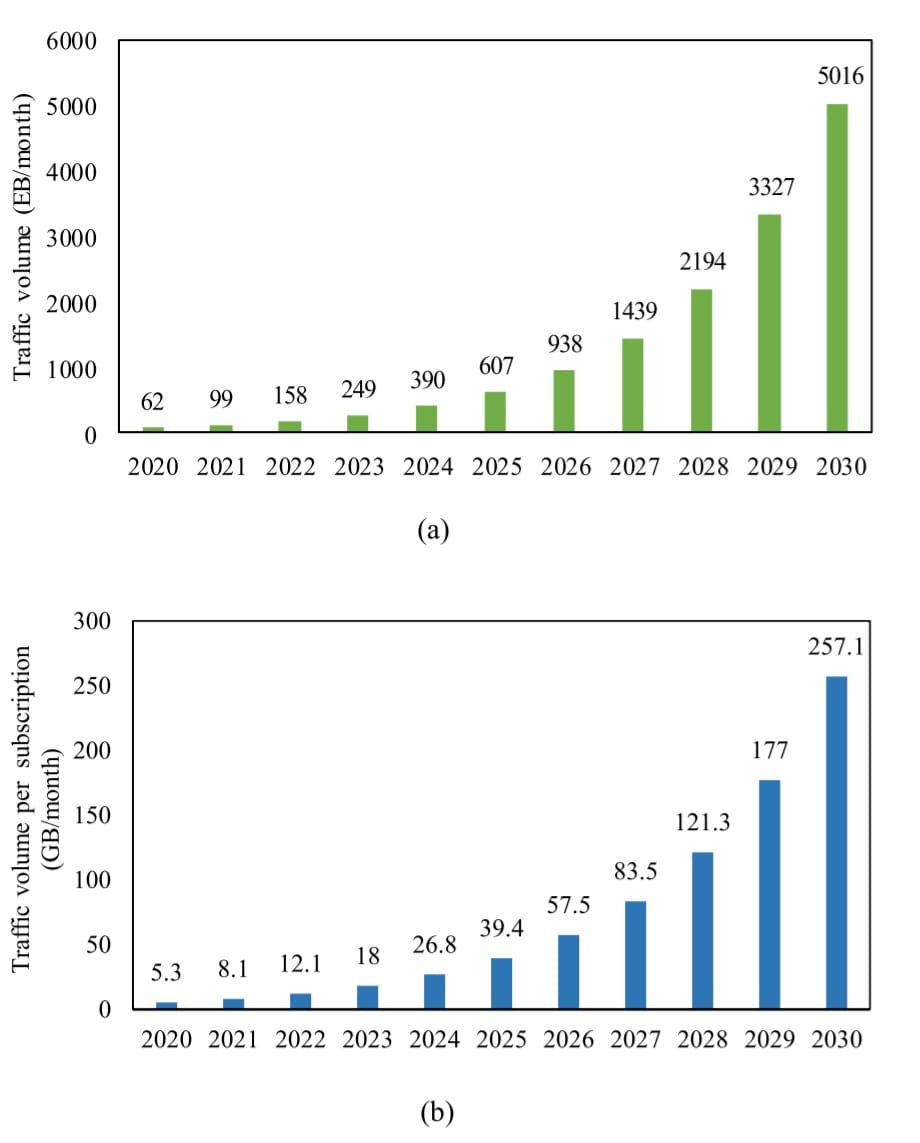
\includegraphics[width=\linewidth]{graph.jpg}

        % Right column for text
        \column{0.56\textwidth}
        
        % First block of text
        \textcolor{red}{\underline{\textbf{Total Global Traffic Volume(EB/month)}}}:-
        \textcolor{green}{GREEN BARS}
        \begin{itemize}
            \item 2020: 62 EB → 2030: 5016 EB (≈80× growth in 10 years)
            \item Driven by IoT, XR, AI, cloud gaming, autonomous systems
        \end{itemize}

        % Second block of text
        \vspace{0.5em} % small spacing between two sections
        \textcolor{red}{\underline{\textbf{Traffic per Subscription (GB/month)}}}:-
        \textcolor{blue}{BLUE BARS}
        \begin{itemize}
            \item 2020: 5.3 GB → 2030: 257.1 GB (≈50× growth per user)
            \item Growth from ultra-HD video, VR/AR, AI-driven services
        \end{itemize}

    \end{columns}
\end{frame}


\begin{frame}{COMPARISON OF 6G WITH 4G AND 5G COMMUNICATION SYSTEMS}
    \resizebox{\textwidth}{!}{%
        \begin{tabular}{|l|c|c|c|}
            \hline
            \textbf{Issue} & \textbf{4G} & \textbf{5G} & \textbf{6G} \\
            \hline
            Per device peak data rate & 1 Gbps & 10 Gbps & 1 Tbps \\
            End-to-end (E2E) latency  & 100 ms & 10 ms  & 1 ms \\
            Maximum spectral efficiency & 15 bps/Hz & 30 bps/Hz & 100 bps/Hz \\
            Mobility support & Up to 350 km/hr & Up to 500 km/hr & Up to 1000 km/hr \\
            Satellite integration & No & No & Full \\
            AI & No & Partial & Full \\
            Autonomous vehicle & No & Partial & Full \\
            XR & No & Partial & Full \\
            Haptic Communication & No & Partial & Full \\
            THz communication & No & Very limited & Full \\
            Service level & Video & VR, AR & Tactile Internet \\
            Architecture & MIMO & Massive MIMO & Intelligent Surfaces \\
            Maximum frequency & 6 GHz & 90 GHz & 1 THz \\
            \hline
        \end{tabular}
    }
\end{frame}


\begin{frame}{Arc} % plain removes header/footer
    \begin{tikzpicture}[remember picture,overlay]
        \node[at=(current page.center),inner sep=0pt] {
            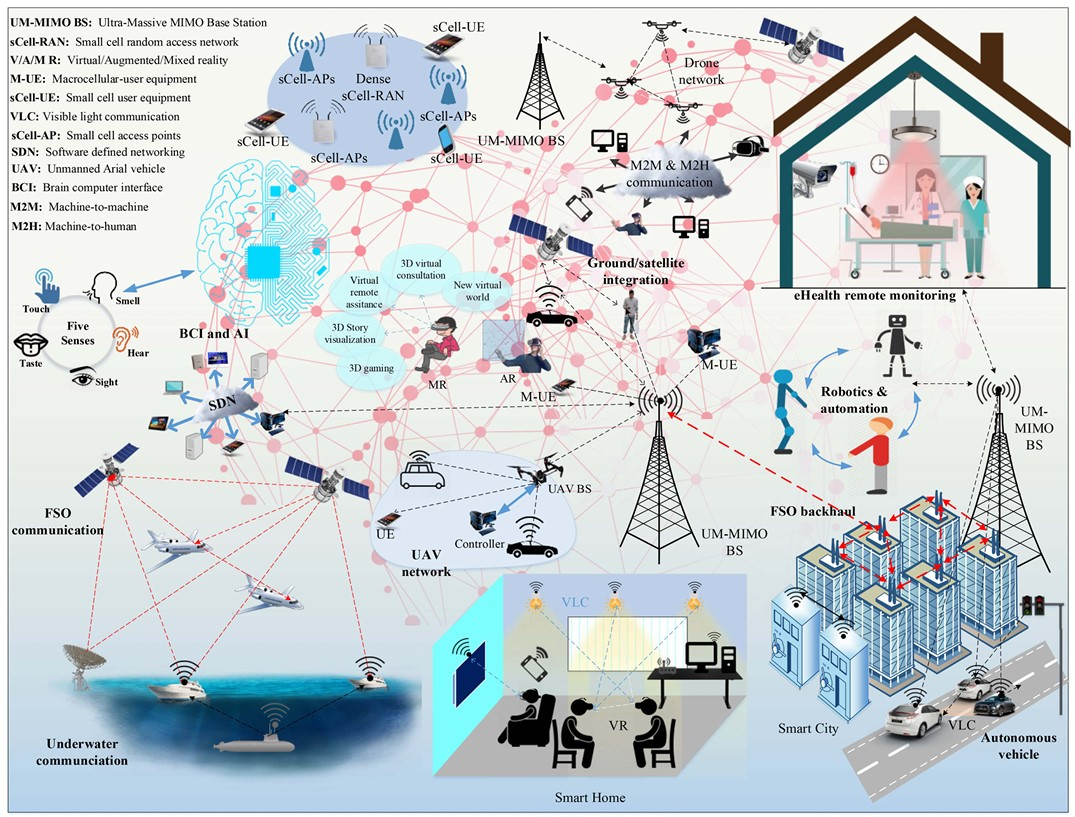
\includegraphics[width=\paperwidth,height=\paperheight]{arc.jpg}
        };
    \end{tikzpicture}
\end{frame}

\begin{frame}{FUNDAMENTAL ENABLING TECHNOLOGIES OF 6G}
\begin{itemize}
    \item Terahertz (THz) Communication
    \item Massive MIMO \& Intelligent Surfaces
    \item Artificial Intelligence (AI) \& Machine Learning (ML)
    \item Quantum Communication \& Computing
    \item 3D Networking \& Integration
    \item Edge Computing \& Cloud Integration
    \item Blockchain \& Security Technologies
\end{itemize}   
\end{frame}

\begin{frame}{STANDARDIZATION AND RESEARCH ACTIVITIES IN 6G}
\begin{itemize}
    \item International Telecommunication Union (ITU)
    \item 3rd Generation Partnership Project (3GPP)
    \item Next G Alliance (North America)
    \item Hexa-X Project (Europe)
    \item 6G Flagship (Finland)
    \item China, Japan, South Korea
    \item India’s 6G Mission
\end{itemize}
\end{frame}

\begin{frame}{Challenges and Future Research Directions in 6G}
\begin{columns}[T] 

\begin{column}{0.48\textwidth}
 \textcolor{red}{\underline{\textbf{Challenges}}}
\begin{itemize}
    \item \textbf{Spectrum Scarcity} 
    \item \textbf{Hardware Limitations} 
    \item \textbf{High Energy Consumption} 
    \item \textbf{Security \& Privacy} 
    \item \textbf{Deployment Costs} 
\end{itemize}
\end{column}

\begin{column}{0.48\textwidth}
 \textcolor{blue}{\underline{\textbf{Future Research Directions}}}
\begin{itemize}
    \item \textbf{Terahertz Communication Systems}
    \item \textbf{AI-Native Networking} 
    \item \textbf{Sustainable 6G} 
    \item \textbf{Integrated Sensing and Communication (ISAC)} 
    \item \textbf{Quantum Communication \& Security} 
    \item \textbf{3D Global Coverage} 
    \item \textbf{Holographic \& Immersive Applications} -
\end{itemize}
\end{column}
\end{columns}
\end{frame}

\begin{frame}{CONCLUSION}
\begin{itemize}
    \item \textbf{6G will redefine connectivity} with ultra-high data rates, ultra-low latency, and global coverage.
    \item Integration of \textbf{AI, Terahertz bands, quantum security, and intelligent surfaces} will make networks smarter and more reliable.
    \item Major challenges in \textbf{spectrum, cost, sustainability, and security} demand continuous innovation.
    \item Ongoing \textbf{global research and standardization efforts} are shaping the roadmap toward IMT-2030.
    \item 6G is not just faster internet -- it is the foundation for \textbf{holograms, digital twins, and intelligent societies}.
\end{itemize}

\vspace{0.4cm}
\centering
\textcolor{green}{\textbf{\Large ``6G – Connecting Intelligence Everywhere''}}
\end{frame}

\begin{frame}{References}
\begin{footnotesize}
\begin{enumerate}
    \item S. Mumtaz et al., “Terahertz communication for vehicular networks,” 
    \textit{IEEE Trans. Veh. Technol.}, vol. 66, no. 7, pp. 5617–5625, Jul. 2017.
    
    \item “IMT traffic estimates for the years 2020 to 2030,” 
    \textit{Int. Telecommun. Union}, ITU-Recommendation M.2370-0, Jul. 2015.
    
    \item S. J. Nawaz, S. K. Sharma, S. Wyne, M. N. Patwary, and M. Asaduzzaman, 
    “Quantum machine learning for 6G communication networks: State-of-the-art and vision for the future,” 
    \textit{IEEE Access}, vol. 7, pp. 46317–46350, 2019.
    
    \item M. Giordani, M. Polese, M. Mezzavilla, S. Rangan, and M. Zorzi, 
    “Toward 6G networks: Use cases and technologies,” 
    \textit{IEEE Commun. Mag.}, vol. 58, no. 3, pp. 55–61, Mar. 2020.
    
    \item M. Shafi et al., “5G: A tutorial overview of standards, trials, challenges, deployment, and practice,” 
    \textit{IEEE J. Sel. Areas Commun.}, vol. 35, no. 6, pp. 1201–1221, Jun. 2017.
    
    \item D. Zhang, Z. Zhou, S. Mumtaz, J. Rodriguez, and T. Sato, 
    “One integrated energy efficiency proposal for 5G IoT communications,” 
    \textit{IEEE Internet Things J.}, vol. 3, no. 6, pp. 1346–1354, Dec. 2016.
    
    \item M. Jaber, M. A. Imran, R. Tafazolli, and A. Tukmanov, 
    “5G backhaul challenges and emerging research directions: A survey,” 
    \textit{IEEE Access}, vol. 4, pp. 1743–1766, 2016.
\end{enumerate}
\end{footnotesize}
\end{frame}

\begin{frame}{Arc}
    \begin{tikzpicture}[remember picture,overlay]
        \node[at=(current page.center),inner sep=0pt] {
            
\includegraphics[width=\paperwidth,height=\paperheight]{th.jpg}
        };
    \end{tikzpicture}
\end{frame}


\end{document}


